\documentclass[uplatex,12pt]{jsarticle}
\usepackage[dvipdfmx]{graphicx}
\usepackage{url}
\usepackage{listings,jlisting}
\usepackage{ascmac}
\usepackage{amsmath,amssymb}

%ここからソースコードの表示に関する設定
\lstset{
  basicstyle={\ttfamily},
  identifierstyle={\small},
  commentstyle={\smallitshape},
  keywordstyle={\small\bfseries},
  ndkeywordstyle={\small},
  stringstyle={\small\ttfamily},
  frame={tb},
  breaklines=true,
  columns=[l]{fullflexible},
  numbers=left,
  xrightmargin=0zw,
  xleftmargin=3zw,
  numberstyle={\scriptsize},
  stepnumber=1,
  numbersep=1zw,
  lineskip=-0.5ex
}
%ここまでソースコードの表示に関する設定

\title{知能プログラミング演習II 課題5}
\author{グループ8\\
  29114060 後藤 拓也\\
}
\date{2019年12月9日}

\begin{document}
\maketitle

\paragraph{提出物} rep5
\paragraph{グループ} グループ8

\paragraph{メンバー}
\begin{tabular}{|c|c|c|}
  \hline
  学生番号&氏名&貢献度比率\\
  \hline\hline
  29114003&青山周平&No\\
  \hline
  29114060&後藤拓也&No\\
  \hline
  29114116&増田大輝&No\\
  \hline
  29114142&湯浅範子&No\\
  \hline
  29119016&小中祐希&No\\
  \hline
\end{tabular}



\section{課題の説明}
\begin{description}
\item[必須課題5-1] 目標集合を変えてみたときに,動作が正しくない場合があったかどうか,実行例を示して考察せよ.
また,もしあったならその箇所を修正し,どのように修正したか記せ.
\item[必須課題5-2] 教科書のプログラムでは,オペレータ間の競合解消戦略としてランダムなオペレータ選択を採用している.
これを,効果的な競合解消戦略に改良すべく考察し,実装せよ.
改良の結果,性能がどの程度向上したかを定量的に(つまり数字で)示すこと.
\item[必須課題5-3] 上記のプランニングのプログラムでは,ブロックの属性(たとえば色や形など)を考えていないので,色や形などの属性を扱えるようにせよ.ルールとして表現すること.
例えば色と形の両方を扱えるようにする場合,Aが青い三角形,Bが黄色の四角形,Cが緑の台形であったとする.
その時,色と形を使ってもゴールを指定できるようにする("green on blue" や"blue on box"のように)
\item[必須課題5-4] 上記5-2, 5-3で改良したプランニングシステムのGUIを実装せよ.
ブロック操作の過程をグラフィカルに可視化し,初期状態や目標状態をGUI上で変更できることが望ましい.
\item[発展課題5-5] ブロックワールド内における物理的制約条件をルールとして表現せよ.
例えば,三角錐(pyramid)の上には他のブロックを乗せられない等,その世界における物理的な制約を実現せよ.
\item[発展課題5-6] ユーザが自然言語(日本語や英語など)の命令文によってブロックを操作したり,初期状態/目標状態を変更したりできるようにせよ.
なお,命令文の動詞や語尾を1つの表現に決め打ちするのではなく,多様な表現を許容できることが望ましい.
\item[発展課題5-7] 3次元空間 (実世界) の物理的な挙動を考慮したブロックワールドにおけるプランニングを実現せよ.
なお,物理エンジン等を利用する場合,Java以外の言語のフレームワークを使って実現しても構わない.
\item[発展課題5-8] 教科書3.3節のプランニング手法を応用できそうなブロック操作以外のタスクをグループで話し合い,新たなプランニング課題を自由に設定せよ.
さらに,もし可能であれば,その自己設定課題を解くプランニングシステムを実装せよ.
\end{description}

\section{発展課題5-6}
\begin{screen}
ユーザが自然言語(日本語や英語など)の命令文によってブロックを操作したり,初期状態/目標状態を変更したりできるようにせよ.
なお,命令文の動詞や語尾を1つの表現に決め打ちするのではなく,多様な表現を許容できることが望ましい.
\end{screen}
\subsection{手法}
ユーザの命令によるブロック操作を行う際, 何も考えずにただ漠然とブロックを動かしていては, プランニングの意味をなさない. 例えば「ブロックをA, B, Cの順に上から積んでいく」という目標が設定されている場合, オペレータは「Cの上にBを置く」のちに「Bの上にAを置く」とするのが理想であり, プランニングではその処理を行えなければならない. ここでユーザが「Cの上にAを置く」などでたらめなことをしてしまっては, プランニングの意味がない. そのため, ここにおける"ユーザによるブロック操作"の定義を, "プランニングを行っているユーザによるブロック操作"とする. \\
具体的には, プログラムが"おすすめ"の操作をユーザに知らせる. ユーザはそのおすすめを参考に処理を選択し, 実行する. もちろんユーザはプランニングを行っているという仮定のもとでの話なので, 条件に合わないオペレータ選択(つまり, 現在の目標に関わる内容がオペレータのAdd-listに存在しない)場合は, そのユーザの選択はプランニングにそぐわないとして実行されず, 代わりにおすすめの処理が行われるとする.\\
プログラムが勧める"おすすめ"のオペレータとは, 課題5-2で行った競合解消戦略によるオペレータ選択の内容である.\\


ここで問題となるのは, オペレータを4つの中から選択できたとしても, 中身までは選択できない...よね...う~ん...
ユーザの選択をどこまで許すかという点である. 上記の例をもう一度考えると, 副目標「B on C」に対して, 「A on C」という処理は, 行えな...いかな...んんn( ,,`・ω・´)ンンン?


ブロック操作における競合解消戦略として, 教科書のプログラムではランダム関数を用いたオペレータの選択をしているが, その選択を適切に変える. 以下の2つの操作を試みている.

\begin{enumerate}
\item 推論の最中にユーザーの入力により, オペレータをその都度選択していく
\item ゴール状態と現在の状態を比べてより最適なオペレータを選択する
\end{enumerate} 

この推論システムは大きく, plannnigメソッドとplannigAGoalメソッドを再帰的に呼び合うことで成り立っている.
以下の図1を参考にしてほしい.
\begin{figure}[htbp]
 \begin{center}
  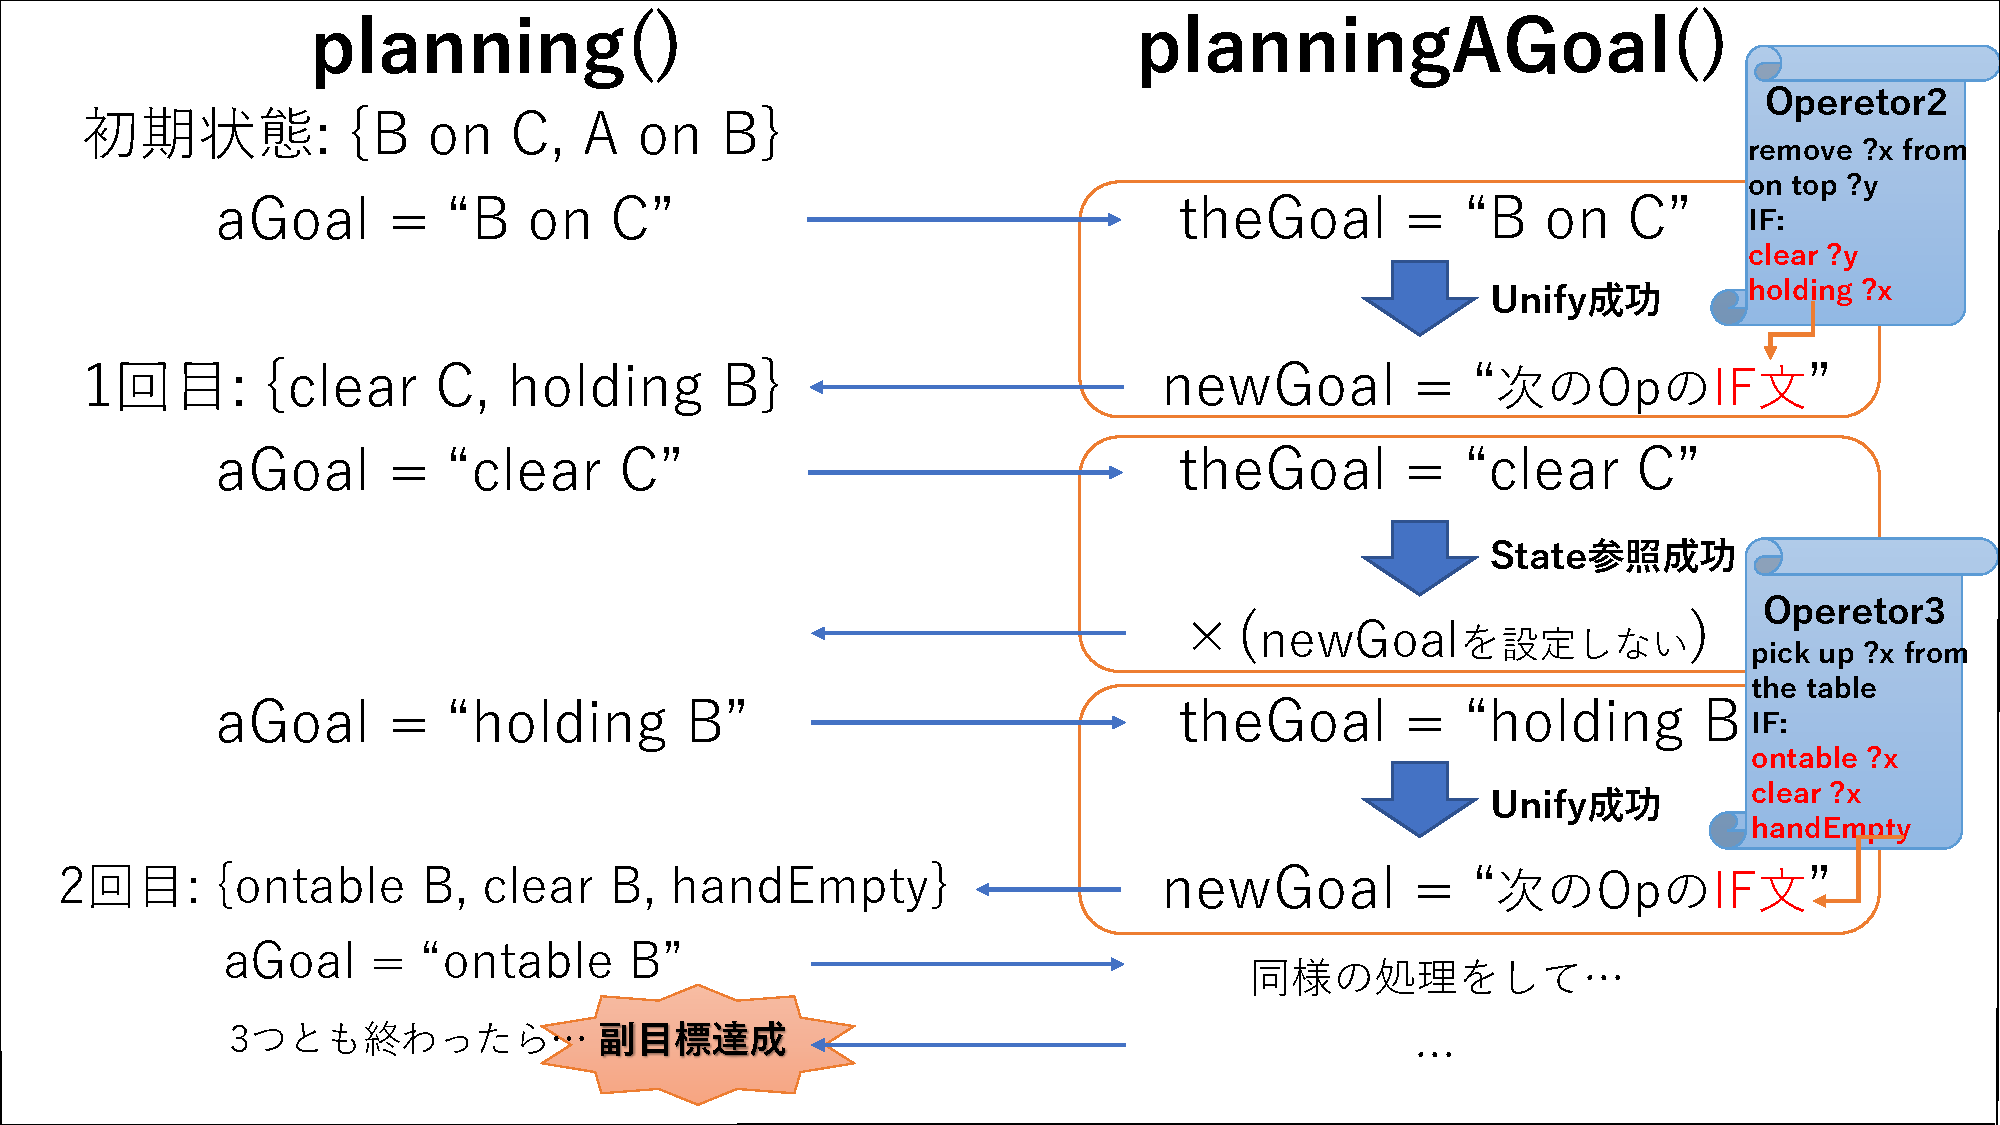
\includegraphics[width = 12cm, pagebox = cropbox, clip]{images/planning.pdf}
 \end{center}
 \caption[]{plannnigにおける相互メソッドの再帰構造}\label{fig:fig1.1}
\end{figure}

plannningAGoalメソッドで, plannnigメソッドから1つ取り出された目標状態を見て, 現状態に含まれていなければ各ルールのAdd-listからUnifyできるオペレータを,  現状態に含まれていればそのまま次の目標へといった流れである. このplanningAGoalメソッドでルールを選ぶ方法をランダムから変えれば良いことが分かる.\\

ランダムにオペレータを選択する際に, 教科書のプログラムは選択したオペレーションを一度, リストから取り除き, その後リストの最後に格納しているが, それだと適切なオペレータを選択できない.

\begin{figure}[htbp]
 \begin{center}
  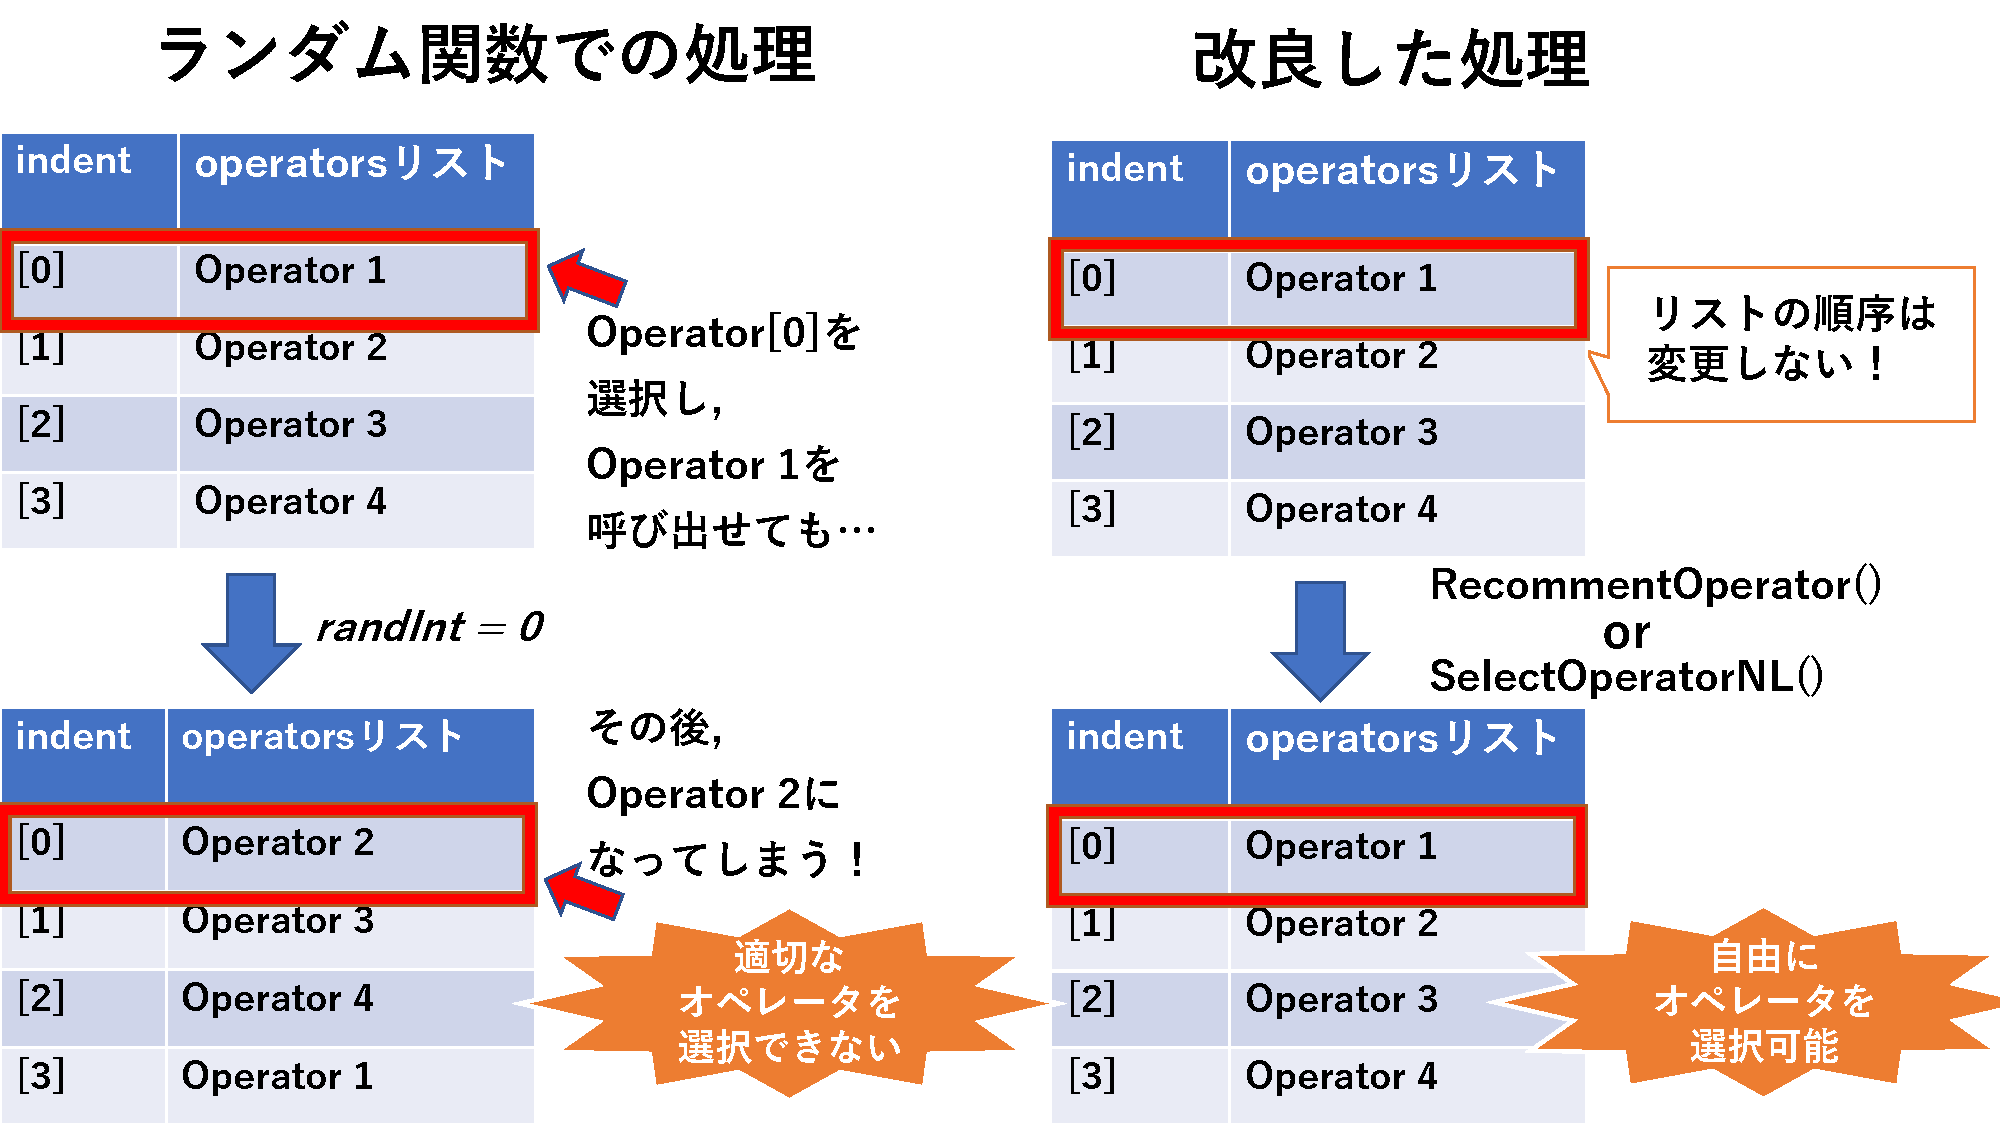
\includegraphics[width = 12cm, pagebox = cropbox, clip]{images/random.pdf}
 \end{center}
 \caption[]{operetarsリストの動き}\label{fig:fig1.1}
\end{figure}

そのため, 図2のように, operatorsリストの順序を適切に扱うことで, 自由にオペレータを選択, 取り出すことにする.


\subsection{実装}
planningAGoalメソッドにおけるオペレータの選択においては, それぞれ新しくメソッドを作成し, そこで適切なオペレータの番号を返すことになっている. 推論の最中にオペレータを選択するSelectOperetorNLメソッドと,, 最適なオペレータ選択をするReccomendOperetorメソッドを作成した.
\begin{lstlisting}[caption=オペレータ選択, label=src:No1]
	//1.ランダム用
	int randInt = Math.abs(rand.nextInt()) % operators.size();
  	Operator op = (Operator)operators.get(randInt);
	operators.remove(randInt);
	operators.add(op);
	//cPoint = randInt;

	//2.発展課題5-6用
	//int numOp = SelectOperatorNL();

	//3.その他開発用
	int numOp = RecommentOperator(theGoal);

	/* 2.3のどちらかを使うときは,このコメントアウトを外してね!
	Operator op = (Operator)operators.get(numOp);
	System.out.println("オペレータ内容は = " + op.name);
	System.out.println("Thank you!");
	cPoint = numOp;
\end{lstlisting}



\begin{lstlisting}[caption=推論中におけるオペレータ選択, label=src:No1]
     /*
	* 自然言語の命令によってオペレータの選択
	*  return オペレータの番号
	*/
	private int SelectOperatorNL() {
		int opNumber = 0;
		Scanner scanner = new Scanner(System.in);
		System.out.println("数値を入力してください。");
		opNumber = scanner.nextInt();
	 	return	opNumber;
	}

\end{lstlisting}
現状はただオペレータの数値を入力することしかできていない. この仮引数にString型の自然言語をもち, その内容からオペレータを選択できるようにしていこう. 

\begin{lstlisting}[caption=最適なオペレータ選択, label=src:No1]
     /*
	* 最適な操作をできるようなオペレータの選択
	*  仮引数  : theGoalの内容
	*  return: オペレータの番号
	*/
	private int RecommentOperator(String theGoal) {
		int opNumber = 0;
		if(theGoal.contains("on")) {
			opNumber = 0;
		}
		else if(theGoal.contains("holding")) {
			opNumber = 2;
		}
		return opNumber;
	}
\end{lstlisting}

現状は上に積むことしか考えていないので,  「A on B」のような目標では, 必ずオペレータの0番目「Place ?x on ?y」を選択し, 「holding A」の目標では, 必ず2番目のオペレータ「pick up ?x from the table」を選択するようになっている.

\subsection{実行例}
最終的なプランニングの結果を以下に示す.\\
以下はランダムなオペレータの選択をしている.
\begin{lstlisting}
***** This is a plan! *****
pick up B from the table
Place B on A
remove B from on top A
Place B on A
remove B from on top A
Place B on A
remove B from on top A
Place B on C
pick up A from the table
Place A on B
\end{lstlisting}

次にオペレータ選択をチューニングした最適なプランニングを示す.
\begin{lstlisting}
***** This is a plan! *****
pick up B from the table
Place B on A
remove B from on top A
Place B on A
remove B from on top A
Place B on A
remove B from on top A
Place B on C
pick up A from the table
Place A on B
\end{lstlisting}

\subsection{考察}

\subsection{感想}
出力結果とプログラムを理解していくのがとても大変であった. 初期プログラムの出力だけでは, なにが起こっているのか全く分からない. 分岐箇所やメソッドに結果などを細かく出力していくことで, プログラムを解読できた.

%%%%%%%%%%%%%%%%%% 参考文献 %%%%%%%%%%%%%%%%%%%%%%%%%%%%%%%%%%%%%%%
\begin{thebibliography}{99}
\bibitem{notty} Javaによる知能プログラミング入門 --著:新谷 虎松 \\
\end{thebibliography}

\end{document}